\documentclass[11pt]{article}

% First load extension packages
\usepackage[a4paper,margin=12.5mm]{geometry}    % page layout
\usepackage{setspace} \onehalfspacing         % line spacing
\usepackage{amsfonts,amssymb,amsmath}         % useful maths extensions
\usepackage{graphicx}                         % graphics import
\usepackage{siunitx}                          % easy SI units
\usepackage{cite}                             % better citations
\usepackage{hyperref}                         % hyperlinking
\usepackage{float}
\usepackage{adjustbox}
\usepackage{booktabs}
\usepackage{tabularx}
\usepackage{makecell}
\usepackage{tikz}
\usetikzlibrary{shapes.geometric, arrows.meta, positioning}
\newcolumntype{Y}{>{\raggedright\arraybackslash}X}
\newcolumntype{Z}{>{\raggedright\arraybackslash}X}

% Change paragraph indentation
\setlength{\parskip}{12pt}
\setlength{\parindent}{0pt}

% User-defined commands
\newcommand{\diff}[2]{\frac{\mathrm{d}{#1}}{\mathrm{d}{#2}}}
\newcommand{\ddiff}[2]{\frac{\mathrm{d}^2{#1}}{\mathrm{d}{#2}^2}}
\newcommand{\pdiff}[2]{\frac{\partial{#1}}{\partial{#2}}}
\newcommand{\pddiff}[2]{\frac{\partial^2{#1}}{\partial{#2}^2}}
\newcommand{\pdiffdiff}[3]{\frac{\partial^2{#1}}{\partial{#2}\partial{#3}}}
\renewcommand{\vec}[1]{\boldsymbol{#1}}
\newcommand{\Idx}{\;\mathrm{d}x}
\newcommand{\Real}{\mathbb{R}}
\newcommand{\Complex}{\mathbb{C}}
\newcommand{\Rational}{\mathbb{Q}}
\newcommand{\Integer}{\mathbb{Z}}
\newcommand{\Natural}{\mathbb{N}}

% topmatter
\title{Cognitive AI Coursework:  Integrating brain-inspired constraints in neural network models.}
\author{Dan Padian}
\date{\today}

% main body
\begin{document}
\maketitle

\tableofcontents
\newpage

%=============================================================================
% QUESTION 1: CRITICAL DISCUSSION (Max 4 pages total for a, b, c, d)
%=============================================================================
\section{Question 1: Brain-Inspired Constraints in Neural Networks}
\label{sec:question1}

% Critically discuss how changes to architecture, cost function, learning rule,
% and other factors can impose brain-like constraints on ANNs.
% Use equations and figures where helpful.
% Max 4 pages TOTAL for all subsections combined.

%-----------------------------------------------------------------------------
\subsection{Architecture [5 marks]}
\label{sec:q1_architecture}

Architectural modifications impose biologically grounded constraints by altering the structure and dynamics of artificial neural networks (ANNs). Whereas standard ANNs prioritise flexibility and ease of optimisation, biologically inspired architectures trade some of this flexibility to capture key organisational principles of real neural circuits.

Standard RNNs update their hidden state in discrete steps, which does not fully reflect the continuous, leaky integration of biological neurons. Leaky RNNs address this by introducing a membrane time constant $\tau$ that governs the rate at which activity decays relative to how much new input is incorporated:
\begin{equation}
\label{eq:leaky_rnn}
a(t) = a(t-1) + \frac{\Delta t}{\tau}\Big[-a(t-1) + f\big(W_{x \to a} x(t) + W_{a \to a} a(t-1) + b_1\big)\Big].
\end{equation}
The parameter $\tau$ therefore sets the effective temporal scale of each unit: smaller values produce fast, input-driven dynamics, whereas larger values enable slow, sustained integration. This mirrors functional differences observed in the brain, where sensory areas respond rapidly to changing inputs while higher-order regions integrate information over longer timescales for working memory and decision-making.

A second biological principle is Dale's law, which states that a neuron is either exclusively excitatory or exclusively inhibitory across all its outputs \cite{Song2016}. This can be implemented by enforcing fixed weight signs after each update:
\begin{equation}
\label{eq:dales_law}
W^{\text{rec}} = W^{\text{rec},+} \odot D,
\end{equation}
where $W^{\text{rec},+}$ is the rectified recurrent weight matrix and $D$ is a diagonal matrix with $D_{ii}=+1$ for excitatory units and $D_{ii}=-1$ for inhibitory units. Typical cortical ratios (e.g., 80\% excitatory, 20\% inhibitory) may be used or adjusted depending on the targeted brain region. Enforcing Dale’s law promotes excitatory--inhibitory balance and prevents units from arbitrarily switching signs, thereby encouraging stable recurrent computation through coordinated population dynamics.

Finally, biological neural circuits exhibit sparse connectivity: cortical neurons synapse onto only a small fraction of their potential targets (often $\sim20\%$). This can be modelled using binary masks:
\begin{equation}
W^{\text{rec}}_{\text{sparse}} = W^{\text{rec}}_{\text{dense}} \odot M,
\end{equation}
where $M_{ij} \in \{0,1\}$ specifies which connections are permitted. Sparse connectivity reduces the number of free parameters, improves interpretability by making information pathways explicit, and forces the network to develop structured representations under realistic wiring constraints.

In summary, these architectural modifications capture three core features of biological computation: temporal integration through membrane time constants, stable dynamics via excitatory--inhibitory balance, and structured information flow enabled by sparse anatomical connectivity.


% Discuss architectural constraints that make networks more brain-like:
% - Leaky integration / time constants
% - Dale's principle (E/I separation)
% - Sparse connectivity
% - Recurrent vs feedforward
% - Cell types and structured connectivity

% Examples:
% - Leaky RNN dynamics
% - E/I neuron separation
% - Sparse masks

% References: Song et al., 2016; Liu & Wang, 2024; course notes Week 4B

%-----------------------------------------------------------------------------
\subsection{Cost Function [5 marks]}
\label{sec:q1_cost}

The cost function is where biological constraints can be imposed most directly, as it dictates which network configurations are preferred during optimisation. By adding appropriate regularisation terms, learning can be steered towards operating regimes that more closely resemble those of biological neural circuits.

As noted in Section~\ref{sec:q1_architecture}, biological networks exhibit sparse connectivity and relatively low firing rates (often $<20$ Hz) due to metabolic constraints. These properties can be encouraged in artificial networks through regularisation penalties. First, L1 regularisation on synaptic weights promotes sparse connectivity \cite{yang2019}:
\begin{equation}
\label{eq:l1_regularization}
J = J_{\text{task}} + \beta_{\text{L1,weight}} \sum_{i,j} |w_{i \to j}|.
\end{equation}
The absolute-value penalty pushes many weights toward zero, yielding connectivity matrices in which only essential links remain. Unlike fixed architectural masks (Section~\ref{sec:q1_architecture}), this approach allows the network to \emph{learn} which connections to prune, with $\beta_{\text{L1,weight}}$ controlling the sparsity--performance trade-off.

Second, L2 regularisation on firing rates captures the metabolic cost of neural activity:
\begin{equation}
\label{eq:l2_regularization}
J = J_{\text{task}} + \beta_{\text{L2,rates}} \sum_{t=1}^{T} \sum_{i=1}^{N} a_{i,t}^2.
\end{equation}
Because activity is penalised quadratically, the network is encouraged to maintain low-amplitude firing while still supporting task-relevant dynamics. This tends to smooth hidden-state trajectories, prevent runaway excitation, and promotes stable recurrent computation.

Biological connectivity is also shaped by spatial structure: empirical studies show that connection probability decays exponentially with physical distance \cite{achterberg2023}. This can be modelled by embedding units in Euclidean space and penalising long-range connections:
\begin{equation}
J = J_{\text{task}} + \beta_{\text{WD}} \sum_{i,j} |w_{i \to j}| \times d_{i \to j},
\end{equation}
where $d_{i \to j}$ is the inter-unit distance. This encourages predominantly local wiring while permitting sparse long-range projections when functionally necessary, mirroring cortical organisation in which short-range connectivity dominates but strategic long-range links support inter-area communication.

Each regularisation term introduces trade-offs: excessively strong L1 penalties can prune connections essential for task performance, whereas weak penalties impose little biological structure; large L2 penalties may suppress necessary transient responses and exacerbate vanishing gradients; and distance-based penalties depend sensitively on the chosen spatial embedding and decay profile. In practice, the $\beta$ hyperparameters must be tuned to balance biological realism against accuracy. Taken together, these cost-function terms provide complementary mechanisms for steering networks toward biologically plausible regimes—enforcing sparse wiring, low metabolic activity, and realistic spatial structure—while remaining fully compatible with gradient-based optimisation.


\subsection{Learning Rule [5 marks]}
\label{sec:q1_learning}

The learning rule determines how synaptic weights change in response to activity and error signals, making it central to biological plausibility. Standard backpropagation suffers from three critical implausibilities: the weight transport problem (requiring $W = W^{\top}$), non-local credit assignment, and for recurrent networks, the \emph{perfect memory problem}—neurons must store and retrieve past activities with unrealistic precision. For temporal tasks, backpropagation through time (BPTT) exacerbates these issues by unrolling networks across dozens of timesteps, demanding that each unit perfectly recall its entire activity history.

Feedback alignment \cite{lillicrap2016} addresses weight transport by replacing $W^{\top}$ with a fixed, randomly initialised feedback matrix $B$:
\begin{equation}
\label{eq:feedback_alignment}
\Delta W \propto B \delta \quad \text{instead of} \quad W^{\top} \delta.
\end{equation}
During training, forward weights gradually align with random feedback pathways, allowing $B\delta$ to approximate true gradients without symmetric connectivity. However, this solves only the weight transport problem; the perfect memory issue remains for recurrent architectures.

For RNNs, Random Feedback Local Online (RFLO) learning \cite{murray2019} provides a biologically plausible alternative to BPTT. Rather than storing exact past activities, RFLO maintains a leaky co-activation trace:
\begin{equation}
p_{ab}(t) = \frac{1}{\tau}\phi'(u_a(t))h_b(t-1) + \left(1 - \frac{1}{\tau}\right)p_{ab}(t-1),
\end{equation}
where $\tau$ controls decay rate. Weight updates then combine random feedback with this trace: $\Delta W_{ab}(t) = \alpha [B\delta(t)]_a \times p_{ab}(t)$. Because traces decay naturally with the network's intrinsic timescale, RFLO eliminates both weight transport and perfect memory requirements while remaining local and online. Performance approaches BPTT for moderate temporal dependencies ($T = 20\tau$ to $160\tau$) but degrades gracefully for longer sequences—a biologically realistic limitation.

A complementary approach is the dendritic error model \cite{sacramento2018}, which exploits pyramidal neuron compartmentalisation. Dendrites encode error signals ($\delta_2$) while soma maintain activity ($x_2$), yielding:
\begin{equation}
\frac{dW_1}{dt} = \alpha \left( g(x_2) - g(\delta_2) \right) x_1.
\end{equation}
This single-neuron implementation avoids weight transport, non-locality, and separate learning phases—all computations occur simultaneously within anatomically plausible structures.

Each approach trades off constraints: feedback alignment retains global error propagation but removes weight symmetry; RFLO sacrifices long-range temporal credit for local, online computation; dendritic models require specific cellular architecture. Together, they demonstrate that effective learning is possible under realistic biological constraints, though often with reduced capacity for extreme temporal dependencies or very deep hierarchies.

% Discuss biologically plausible learning rules:
% - Weight transport problem in backprop
% - Feedback alignment
% - RFLO (Random Feedback Local Online)
% - Hebbian learning
% - STDP (Spike-Timing-Dependent Plasticity)
% - Three-factor learning rules

% Key issue: Backprop uses W^T which is biologically unrealistic
% Solutions: Random feedback weights, local learning

% References: Lillicrap et al., 2016; Murray, 2019; Whittington & Bogacz, 2019

%-----------------------------------------------------------------------------
\subsection{Other Constraints [5 marks]}
\label{sec:q1_other}

Beyond architectural, cost-function, and synaptic-level mechanisms, the learning paradigm itself imposes additional biological constraints. Three approaches—curriculum learning, three-factor learning rules, and reinforcement learning—capture principles of developmental progression, neuromodulatory control, and reward-driven adaptation that supervised backpropagation alone cannot model.


Biological learners acquire abilities gradually, mastering simpler behaviours before more complex ones. Curriculum learning formalises this by presenting training examples in an ordered progression—from short, high signal-to-noise sequences to longer or noisier inputs as training stabilises. This staged exposure encourages robust representations, reduces early overfitting, and mirrors developmental trajectories in which sensory systems mature before higher-order cortical areas.

Hebbian plasticity alone is indiscriminate: correlated activity always drives synaptic change. In the brain, plasticity is gated by neuromodulators such as dopamine and acetylcholine, which determine whether correlation leads to lasting modifications \cite{fremaux2016neuromodulated,kusmierz2017learning}. This can be expressed as
\begin{equation}
\dot{w}_{ij} = y \cdot H(\text{pre}_i, \text{post}_j),
\end{equation}
where $y$ is a neuromodulatory signal and $H$ a Hebbian term. Only when $y>0$ does learning occur. Neuromodulatory gradients across cortex \cite{froudist2023gradients} explain why some regions remain highly plastic. In ANNs, this principle is implemented by modulating weight updates with a scalar gating signal linked to reward, salience, or novelty, preventing indiscriminate learning while preserving gradient-based optimisation.


Supervised learning assumes explicit targets—a biologically implausible teaching signal. Reinforcement learning replaces these with scalar rewards, directly paralleling dopaminergic reward prediction error (RPE) signals \cite{schultz1997neural,sutton2018reinforcement}. In temporal-difference learning,
\begin{equation}
V(s_t) \leftarrow V(s_t) + \alpha \big[r_{t+1} + \gamma V(s_{t+1}) - V(s_t)\big],
\end{equation}
the bracketed term corresponds to the RPE encoded by midbrain dopamine neurons. Q-learning extends this to action values:
\begin{equation}
Q(s_t,a_t) \leftarrow Q(s_t,a_t) + \alpha \big[r_{t+1} + \gamma \max_{a'} Q(s_{t+1},a') - Q(s_t,a_t)\big].
\end{equation}
Deep RL methods such as DQN incorporate biologically inspired mechanisms including \emph{experience replay}, akin to hippocampal replay during sleep \cite{wilson1994reactivation}, and stochastic exploration policies reflecting behavioural variability. Model-based RL further aligns with hippocampal–prefrontal interactions supporting planning \cite{wang2018prefrontal}.


Together, these learning-paradigm constraints shape \emph{when}, \emph{how}, and \emph{from what signals} networks learn. Curriculum learning structures difficulty to support gradual skill acquisition; three-factor rules gate plasticity based on behavioural relevance; and reinforcement learning replaces omniscient supervision with sparse rewards that mirror dopaminergic teaching signals. These mechanisms complement earlier architectural and cost-function constraints by aligning training procedures with the temporal, modulatory, and reward-driven nature of biological learning.


%=============================================================================
% QUESTION 2: PRACTICAL IMPLEMENTATION
%=============================================================================
\newpage
\section{Question 2: NeuroGym Task Implementation}
\label{sec:question2}


\subsection{Question 2a: Model Implementation [10 marks / 3 pages]}
\label{sec:question2a}

% Initially, train and compare at least two models:
% 1. Standard RNN (vanilla, leaky, GRU, LSTM)
% 2. Brain-inspired variant(s) based on Q1 discussion

\subsubsection{Task Selection: ReadySetGo}

The ReadySetGo task requires models to measure and reproduce temporal intervals, testing temporal processing capabilities crucial for cognitive function \cite{remington2018flexible}.

\begin{figure}[h]
    \centering
    \includegraphics[width=0.75\textwidth]{figures/readysetgo_task_structure.png}
    \caption{ReadySetGo task structure. Left: Input stimuli showing Ready and Set cues for three trials with different sample intervals.}
    \label{fig:task_structure}
\end{figure}

As shown in Figure \ref{fig:task_structure}, the model receives three inputs: Ready, Set, and fixation signals. The fixation input indicates when to produce the response, whilst Ready and Set cues define the interval to be reproduced. Models must measure the Ready-to-Set interval ($t_s$) and reproduce it scaled by gain factor $g = 1.5$. This requires temporal integration over variable delays (500--2000ms), directly testing the time constants and firing rate regularisation discussed in Question 1. The task mirrors interval timing in prefrontal cortex, isolates temporal processing from working memory demands, and remains sensitive to biological constraints whilst being computationally tractable \cite{remington2018flexible}. 


\subsubsection{Model Architectures}

Before tackling this task four models are defined, progressing from minimal to full biological plausibility with multiple changes to the architecture, cost function and learning rule.

\textbf{Model 1: Vanilla RNN (Baseline)}

To begin with, a standard recurrent architecture with tanh activation, chosen for its bounded output range $[-1, 1]$ that prevents explosive activations whilst allowing both positive and negative values. This serves as the baseline against which biological constraints are evaluated.

\textbf{Model 2: Leaky RNN}

This model incorporates membrane time constant $\tau = 100$ms for temporal integration following Equation~\ref{eq:leaky_rnn} from Section~\ref{sec:q1_architecture}, implementing leaky dynamics where hidden state decay is controlled by $\tau$. Leaky integration allows sustained information maintenance across delays—essential for ReadySetGo's interval timing. Recurrent noise ($\sigma_{\text{rec}} = 0.15$, $\xi_t \sim \mathcal{N}(0,1)$) matches biological neural variability. The activation function switches to ReLU for non-negative firing rates, consistent with biological neurons.

\textbf{Model 3: Leaky RNN + Feedback Alignment}

This model builds on Model 2 by addressing the weight transport problem through feedback alignment \cite{lillicrap2016}, implementing the learning rule from Equation~\ref{eq:feedback_alignment} in Section~\ref{sec:q1_learning} where $\Delta W \propto B \delta$ instead of $W^{\top} \delta$. Forward propagation uses trained weights $W$, whilst backpropagation employs fixed random weights $B$, removing the need for biologically implausible symmetric connectivity whilst maintaining gradient-based learning. The feedback matrix $B$ is initialised uniformly at the scale of forward weights to prevent gradient explosion. 

\textbf{Model 4: Biologically Realistic RNN}

Model 4 integrates four constraints: (1) feedback alignment (Equation~\ref{eq:feedback_alignment}, Section~\ref{sec:q1_learning}), (2) Dale's principle enforcing 80\% excitatory/20\% inhibitory separation via Equation~\ref{eq:dales_law} in Section~\ref{sec:q1_architecture}, (3) L1 weight regularisation ($\beta_{L1} = 10^{-5}$) from Equation~\ref{eq:l1_regularization} in Section~\ref{sec:q1_cost} promoting sparse connectivity, and (4) L2 firing rate regularisation ($\beta_{L2} = 0.01$) from Equation~\ref{eq:l2_regularization} in Section~\ref{sec:q1_cost} enforcing metabolically plausible activity levels. This architecture combines constraints across learning, structure, and optimisation to test whether biological plausibility impairs task performance. 

\textbf{Progressive Architecture Design:}

Figure \ref{fig:model_progression} illustrates the incremental addition of biological constraints across the four architectures. This progressive design enables systematic evaluation of individual constraint contributions: starting from an unconstrained Vanilla baseline, each model adds specific biological mechanisms (temporal integration, biologically plausible learning, structural constraints), allowing isolation of performance trade-offs. This approach directly tests Question 1's theoretical predictions—whether leaky integration (architecture), L1/L2 regularisation (cost function), and feedback alignment (learning rule) can be combined whilst preserving task competence. By comparing adjacent models in the progression, we quantify the cost-benefit trade-off for each biological constraint: Model 2 isolates temporal dynamics' contribution; Model 3 adds learning-rule plausibility; Model 4 tests whether full biological realism (Dale's law, sparsity, metabolic constraints) remains compatible with effective supervised learning.

\begin{figure}[H]
\centering
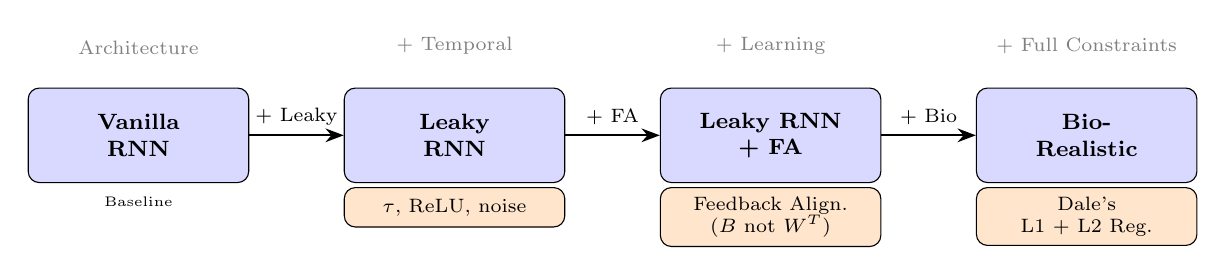
\begin{tikzpicture}[
    model/.style={rectangle, rounded corners, minimum width=2.8cm, minimum height=1.2cm,
                  text centered, draw=black, fill=blue!15, font=\bfseries\footnotesize, align=center},
    constraint/.style={rectangle, rounded corners, minimum width=2.8cm, minimum height=0.5cm,
                       text centered, draw=black, fill=orange!20, font=\scriptsize, align=center},
    arrow/.style={-Stealth, thick, black},
    label/.style={font=\tiny, align=center},
    node distance=0.3cm
]

% Model 1
\node (m1) [model] {Vanilla\\RNN};
\node (c1) [below=0.05cm of m1, label] {Baseline};

% Arrow 1
\node (arrow1) [right=1.2cm of m1] {};
\draw [arrow] (m1) -- node[above, font=\scriptsize] {+ Leaky} (arrow1);

% Model 2 with constraints below
\node (m2) [model, right=1.2cm of m1] {Leaky\\RNN};
\node (m2c) [constraint, below=0.05cm of m2] {$\tau$, ReLU, noise};

% Arrow 2
\node (arrow2) [right=1.2cm of m2] {};
\draw [arrow] (m2) -- node[above, font=\scriptsize] {+ FA} (arrow2);

% Model 3 with constraints below
\node (m3) [model, right=1.2cm of m2] {Leaky RNN\\+ FA};
\node (m3c) [constraint, below=0.05cm of m3] {Feedback Align.\\($B$ not $W^T$)};

% Arrow 3
\node (arrow3) [right=1.2cm of m3] {};
\draw [arrow] (m3) -- node[above, font=\scriptsize] {+ Bio} (arrow3);

% Model 4 with constraints below
\node (m4) [model, right=1.2cm of m3] {Bio-\\Realistic};
\node (m4c) [constraint, below=0.05cm of m4] {Dale's\\L1 + L2 Reg.};

% Top labels
\node[above=0.3cm of m1, font=\scriptsize, text=gray] {Architecture};
\node[above=0.3cm of m2, font=\scriptsize, text=gray] {+ Temporal};
\node[above=0.3cm of m3, font=\scriptsize, text=gray] {+ Learning};
\node[above=0.3cm of m4, font=\scriptsize, text=gray] {+ Full Constraints};

\end{tikzpicture}
\caption{Progressive addition of biological constraints across four model architectures. Each model builds on the previous by adding brain-inspired mechanisms.}
\label{fig:model_progression}
\end{figure}


\subsubsection{Implementation Details}
\label{sec:implementation_models}

All models were trained for 4,000 steps using identical hyperparameters to ensure fair comparison. The Adam optimiser (Kingma \& Ba, 2014) was employed with learning rate $\alpha = 5 \times 10^{-4}$, chosen to balance convergence speed against stability for biologically constrained models where feedback alignment and sparsity penalties can introduce gradient noise. All models use 50 hidden units and batch size 16, with temporal discretisation $\Delta t = 20$ms matching biological spiking timescales. Recurrent noise ($\sigma_{\text{rec}} = 0.15$, $\xi_t \sim \mathcal{N}(0,1)$) is applied only to Leaky-based models (Models 2--4) to match biological neural variability without destabilising the Vanilla baseline.

The loss function combines cross-entropy task loss with biological regularisation terms. Class weights $(0.1, 1.0)$ for fixation versus action outputs address the severe class imbalance inherent in timing tasks—models spend most trial time fixating and respond only briefly at interval end. Without reweighting, networks trivially minimise loss by never responding. For Model 4 (Bio-Realistic), L1 weight regularisation ($\beta_{L1} = 10^{-5}$) and L2 firing rate regularisation ($\beta_{L2} = 0.01$) are added to the task loss following Equations~\ref{eq:l1_regularization} and~\ref{eq:l2_regularization}, encouraging sparse connectivity and metabolically plausible low firing rates. All models implement feedback alignment's fixed random matrix $B$ initialised uniformly at the scale of forward weights to prevent gradient explosion whilst maintaining alignment dynamics.


\subsubsection{Learning Performance}

\begin{figure}[H]
    \centering
    \includegraphics[width=0.75\textwidth]{figures/question_2a_results.png}
    \caption{Learning curves showing task loss only for fair comparison across models. All models successfully learn the timing task to different levels.}
    \label{fig:learning_curves}
\end{figure}

All models successfully converged, achieving task loss below 0.20, indicating that biological constraints are compatible with effective temporal learning. Although all architectures begin learning at similar rates, their trajectories diverge: the bio-realistic model plateaus early at around 0.17, suggesting that feedback alignment and activity regularisation slow convergence relative to standard backpropagation. A similar slowdown appears in the Leaky~+~FA model, consistent with the reduced precision imposed by random feedback weights—a known limitation of biologically plausible learning rules. The vanilla RNN learns reliably but plateaus modestly above the best-performing model. The Leaky RNN shows the strongest performance overall, continuing to improve throughout training and reaching a final task loss of approximately 0.10, suggesting that leaky integration alone provides a powerful inductive bias for interval timing. This aligns with biological evidence that temporal processing relies heavily on slow membrane dynamics even in the absence of additional structural constraints \cite{paton2018neural}.




\newpage
\subsection{Question 2b: Hidden Unit Activity Analysis [20 marks / 4 pages]}
\label{sec:question2b}

% Analyze how trained models solve the task
% Compare models and interpret differences

\subsubsection{Performance Comparison}

Despite similar training losses (<0.20), Figure~\ref{fig:timing_performance} reveals dramatic performance differences. Vanilla (100\% response rate) shows linear scaling but systematic undershooting. Leaky RNN achieves near-perfect performance ($\mu=-19.4$ms, $\sigma=195.5$ms) with $\tau=100$ms enabling accurate temporal integration. Leaky+FA exhibits severe underprediction ($\mu=-324.6$ms, $\sigma=173.2$ms)—feedback alignment impairs temporal mapping whilst preserving task structure (100\% responses). Bio-Realistic displays bimodal behaviour: 31\% complete failures (zero-cluster) and 69\% delayed responses ($\mu=203.6$ms, $\sigma=873.7$ms), revealing that extreme sparsity ($\sim$9 neurons) creates critical dependencies. This 31\% failure rate vastly exceeds biological regimes ($\sim$5--10\% lapses \cite{remington2018}), demonstrating over-constraint beyond cortical sparsity levels.

\begin{figure}[H]
    \centering
    \includegraphics[width=0.9\textwidth]{figures/readysetgo_timing.png}
    \caption{Timing performance analysis across models. \textbf{Left:} Scatter plot showing target versus produced intervals, with black diagonal indicating perfect timing. Leaky RNN (orange) clusters near-perfectly along the diagonal, whilst Leaky+FA (green) systematically undershoots and Bio-Realistic (red) shows high variance with failure modes. \textbf{Right:} Error distributions with mean ($\mu$) and standard deviation ($\sigma$) revealing systematic biases and precision differences. Fixed 50ms bin width enables direct comparison across models.}
\label{fig:timing_performance}
\end{figure}

\subsubsection{Neural Population Dynamics}

PCA trajectories (Fig.~\ref{fig:trajectories}) reveal distinct computational strategies. Vanilla RNN exhibits a single trajectory (PC1: 70.4\%), suggesting fixed attractor dynamics unable to flexibly encode multiple intervals. Leaky RNN shows 10--15 parallel trajectories (PC1: 62.1\%), resembling primate prefrontal dynamics \cite{remington2018} where intervals occupy separate manifold paths. Leaky+FA displays similar structure but higher compression (PC1: 84.2\%)—feedback alignment regularises to lower dimensionality, explaining timing bias through reduced interval discrimination. Bio-Realistic exhibits irregular, jagged trajectories (PC1: 86.6\%) from sparse, intermittent activity mirroring biological recordings \cite{remington2018}; high PC1 variance reflects sparsity, not low dimensionality. Critically, Ready and Go occupy consistent state-space regions whilst Set positions vary, indicating geometric temporal encoding: manifold position directly represents elapsed time—a population clock mechanism \cite{remington2018}.

\begin{figure}[H]
    \centering
    \includegraphics[width=0.9\textwidth]{figures/readysetgo_trajectories.png}
    \caption{Neural trajectories in PCA space (10 trials per model). Green circles mark Ready (trial start), blue diamonds mark Set (cue), red squares mark Go (response).}
    \label{fig:trajectories}
\end{figure}

\subsubsection{Neural Activity Patterns and Functional Specialization}

Activity heatmaps (Fig.~\ref{fig:heatmaps}) and neuron importance rankings (Fig.~\ref{fig:neuron_importance}) reveal distinct sparsity gradients and specialization strategies. Vanilla shows dense sustained firing ($\sim$35 neurons active) with binary patterns—distributed coding lacking temporal precision. Leaky RNN maintains dense activity with structured bursts; Leaky+FA concentrates firing around Set. Bio-Realistic activates only $\sim$9 neurons near Set (18\% sparsity matching cortical 10--20\% \cite{remington2018}), with top 10 neurons dominating variance rankings, forming a specialized "timing circuit". This extreme concentration is metabolically faithful but fragile: reliance on critical neurons explains 31\% response failures.

\begin{figure}[H]
    \centering
    \includegraphics[width=0.9\textwidth]{figures/readysetgo_heatmaps.png}
    \caption{Activity heatmaps showing 50 neurons over time for a single trial across models. Cyan dashed line marks Set cue, lime dashed line marks expected Go response. Vertical axis: neuron index, horizontal axis: time, color: activity magnitude. }
    \label{fig:heatmaps}
\end{figure}

\textbf{Ramping Dynamics.} Individual neuron activity reveals interval timing's canonical signature: linear ramping during Ready→Set. Leaky RNN neurons 15--30 show firing rates increasing linearly with slopes proportional to sample duration, confirming leaky integration implements temporal accumulation ($\tau=100$ms) rather than discrete states \cite{remington2018}. Vanilla shows weak ramping with abrupt transitions, explaining underprediction. Bio-Realistic exhibits irregular, noisy ramping reflecting stochastic sparse recruitment. Ramping neurons maintain elevated activity until Go (working memory), whilst separate units show transient Set/Go bursts, indicating integration-readout specialization. Importance rankings confirm this hierarchy mirrors biological cortex where sparse task-encoding neurons sit within larger populations, exposing the computational trade-off: extreme specialization (Bio-Realistic) is efficient but fragile; distributed coding (Vanilla) is robust but metabolically costly; intermediate strategies (Leaky) balance precision and redundancy.

\begin{figure}[H]
    \centering
    \includegraphics[width=0.9\textwidth]{figures/mechanism_5_neuron_importance.png}
    \caption{Neuron importance ranked by normalized activity variance across time. Bio-Realistic (red) shows extreme concentration with top 10 neurons dominating, whilst Vanilla (blue) distributes computation broadly across ~35 neurons. Leaky models (orange, green) show intermediate specialization, balancing efficiency and robustness.}
    \label{fig:neuron_importance}
\end{figure}

\subsubsection{Validation of Question 1 Predictions}

Empirical findings validate Question 1's constraint taxonomy. \textbf{Architecture:} Leaky integration ($\tau=100$ms, Equation~\ref{eq:leaky_rnn}) enables sustained accumulation—ramping confirms time constants support working memory over 500--2000ms intervals ($\mu=-19.4$ms). Vanilla's lack of $\tau$ produces systematic underprediction. Dale's law (Equation~\ref{eq:dales_law}) contributes stochasticity but permits learning. \textbf{Cost Function:} L1 regularization (Equation~\ref{eq:l1_regularization}) enforces sparsity (18\% active neurons) but introduces fragility (31\% failures), confirming the efficiency-robustness trade-off. L2 regularization (Equation~\ref{eq:l2_regularization}) prevents runaway activity. \textbf{Learning Rule:} Feedback alignment (Equation~\ref{eq:feedback_alignment}) produces systematic bias ($\mu=-324.6$ms) and compresses dimensionality (PC1: 84.2\% vs 62.1\%), confirming temporal credit assignment limitations. All models achieved loss $<0.20$, demonstrating biological constraints permit effective learning with predictable trade-offs.

\subsubsection{Comparison to Biological Neural Data}

Quantitative comparison to primate prefrontal cortex \cite{remington2018} shows Bio-Realistic matches biological sparsity (18\% vs 10--20\% active neurons) and dimensionality (PC1: 86.6\% vs 70--80\%), but exceeds biological noise ($\sigma=873.7$ms vs 150--300ms) and failure rates (31\% vs 5--10\%). Leaky RNN's timing precision ($\sigma=195.5$ms) falls within biological range whilst maintaining moderate constraints, suggesting time constants and moderate regularization capture essential principles without over-constraining capacity. Bio-Realistic's extreme sparsity ($\beta_{L1}=10^{-5}$) pushes beyond biological regimes where redundancy maintains robustness.

\subsubsection{Summary of Findings}

Trained models reveal distinct computational strategies shaped by biological constraints. Leaky RNN achieves optimal performance ($\mu=-19.4$ms) through 10--15 parallel trajectories and moderate specialisation ($\sim$20--30 neurons), balancing precision against robustness. Bio-Realistic's extreme sparsity ($\sim$9 neurons, irregular trajectories) closely resembles primate recordings \cite{remington2018} but introduces fragility: response failures when critical neurons remain silent ($\sigma=873.7$ms). Vanilla's dense coding ($\sim$35 neurons) achieves robustness but sacrifices biological plausibility. Feedback alignment compresses dynamics to lower dimensionality, producing systematic timing bias despite accurate task structure.

Critically, all models encode time geometrically—Set position varies along manifolds whilst Ready and Go occupy consistent regions, implementing population clocks where state-space location represents elapsed time \cite{remington2018}. This convergent solution suggests geometric temporal encoding is fundamental to interval timing. Findings demonstrate biological constraints (Dale's principle, sparse coding, feedback alignment) are compatible with effective learning but introduce specific trade-offs: sparsity improves metabolic efficiency at the cost of fragility, whilst biologically-plausible learning impairs precision even when preserving task accuracy.

%-----------------------------------------------------------------------------
% QUESTION 2C: SECOND TASK (Max 4 pages)
%-----------------------------------------------------------------------------

\newpage
\subsection{Question 2c: Second Task Analysis [20 marks / 4 pages]}
\label{sec:question2c}

To assess whether biological constraints produce task-general computational principles or task-specific solutions, the four architectures are evaluated on \texttt{MultiSensoryIntegration-v0}, a perceptual decision-making task requiring probabilistic evidence accumulation. This contrasts with ReadySetGo's temporal interval reproduction, testing whether architectural differences reflect fundamental constraints or task-dependent adaptations. Multisensory integration tasks model parietal and prefrontal circuits that combine noisy sensory evidence into categorical decisions—a canonical computation studied extensively in neurophysiology \cite{shadlen2001neural}.

\subsubsection{Task Description}

The \texttt{MultiSensoryIntegration-v0} task presents two simultaneous sensory streams (modality 1 and modality 2), each with left/right channels. As shown in Figure \ref{fig:q2_multisensory_task_structure}, inputs comprise five streams: fixation (row 1), mod1-left/right (rows 2--3), and mod2-left/right (rows 4--5). A trial’s difficulty is set by (i) \textbf{coh} -- the evidence strength (higher = cleaner signal, lower = noisy) and (ii) \textbf{coh\_prop} -- the fraction of evidence assigned to modality 1 vs. modality 2 (near 1 biases mod1, near 0 biases mod2). The agent should fixate during the cue, integrate both modalities, and emit a single binary decision (The top row, green=left/red=right) when fixation ends.

\begin{figure}[H]
    \centering
    \includegraphics[width=0.95\textwidth]{figures/q2_multisensory_task_structure.png}
    \caption{Task structure (three concatenated trials): fixation, modality 1 (L/R), modality 2 (L/R), and decision band (green=left, red=right).}
    \label{fig:q2_multisensory_task_structure}
\end{figure}

The network must combine modality-specific evidence (weighted by \textbf{coh\_prop}) and classify left vs. right. Unlike ReadySetGo's sustained temporal integration over variable delays, this requires stateless evidence accumulation—testing whether architectural constraints impose task-general or task-specific computational strategies.

\subsubsection{Training and Performance}

All four architectures were trained identically to ReadySetGo (supervised mode, cross-entropy loss, mini-batches). Loss decays smoothly and stabilises by \(\sim\)8k steps (Fig.~\ref{fig:q2_multisensory_training_curves}), matching ReadySetGo's convergence speed. However, unlike timing where Bio-Realistic plateaued early, all models converge similarly here, suggesting sparse E/I networks handle snapshot decisions better than sustained working memory.

\begin{figure}[H]
    \centering
    \includegraphics[width=0.95\textwidth]{figures/q2_multisensory_training_curves.png}
    \caption{Training loss (log scale) for all architectures; y-lim fixed to 0.05–0.20.}
    \label{fig:q2_multisensory_training_curves}
\end{figure}

\begin{table}[h!]
\centering
\small
\setlength{\tabcolsep}{12pt}
\begin{tabular}{c c c c}
\hline
\textbf{Vanilla RNN} & \textbf{Leaky RNN} & \textbf{Leaky + FA} & \textbf{Bio-realistic} \\
\hline
0.926 & 0.904 & 0.898 & 0.898 \\
\hline
\end{tabular}
\end{table}



All models achieve high accuracy ($>89\%$), contrasting with ReadySetGo where timing precision varied dramatically. Notably, Leaky+FA's severe timing bias ($\mu=-324.6$ms undershoot) disappears here (accuracy 0.898, no directional bias), revealing that feedback alignment impairs temporal credit assignment specifically but handles instantaneous evidence combination effectively—validating Question 1's prediction that biologically plausible learning faces domain-specific limitations. Bio-Realistic shows consistent minor accuracy drops across both tasks, confirming sparsity's task-general performance cost.

\subsubsection{Hidden Unit Analysis}

PCA (Fig.~\ref{fig:q2_multisensory_pca}) reveals dramatically different representational geometry than ReadySetGo. Whereas timing required 10--15 parallel trajectories encoding continuous intervals (PC1: 62.1\%), evidence integration compresses to binary left/right clusters in 2D (Vanilla: $\sim$95\% in PC1--2). This dimensionality difference reflects computational demands: interval timing needs continuous state space where trajectory position encodes elapsed time, whilst categorical decisions collapse evidence onto a single discriminative axis. Bio-Realistic achieves highest PC1 variance in both tasks, confirming that sparsity and E/I balance act as universal dimensionality-reduction mechanisms—a task-general architectural principle. 

\begin{figure}[!h]
    \centering
    \includegraphics[width=0.82\textwidth]{figures/q2_multisensory_pca.png}
    \caption{PCA of per-trial mean hidden states (rows = models, colored by decision).}
    \label{fig:q2_multisensory_pca}
\end{figure}


\begin{figure}[!h]
    \centering
    \includegraphics[width=0.82\textwidth]{figures/q2_multisensory_heatmaps.png}
    \caption{Hidden-unit activity heatmaps (correct trials, averaged) for all models.}
    \label{fig:q2_multisensory_heatmaps}
\end{figure}


Heatmaps (Fig.~\ref{fig:q2_multisensory_heatmaps}) confirm task-invariant sparsity patterns: Bio-Realistic recruits $\sim$10--15 neurons (matching timing's $\sim$9), whilst Vanilla/Leaky activate broadly across both tasks. Critically, temporal dynamics differ—ReadySetGo showed sustained ramping activity, whilst integration exhibits brief bursts near decision windows. This suggests architectural sparsity is task-general (L1/L2 constraints universally enforce metabolic efficiency), but \emph{which} neurons activate and \emph{when} depends on computational demands. Bio's sparse profile echoes cortical recordings but introduces fragility: timing failures (zero-cluster) versus integration accuracy drops both stem from critical neuron dependence.

The distinct temporal profiles validate Question 1's hierarchical time constant principle: evidence integration benefits from fast, transient responses (like sensory V1, $\tau \sim 20$--100ms) for snapshot decisions, whereas ReadySetGo's interval timing demands slow integration ($\tau = 100$ms in our Leaky models) matching prefrontal timescales ($\sim$1--10s). This explains why Bio-Realistic struggled more with timing than integration—sparse E/I circuits with strong feedback alignment may implement distributed decision boundaries effectively (as in parietal cortex multisensory integration \cite{shadlen2001neural}) but lack the sustained recurrent excitation necessary for working memory maintenance without dense connectivity. Dale's principle further constrains solutions: excitatory-excitatory recurrence supports persistent activity in timing tasks \cite{chaudhuri2015}, whilst balanced E/I creates winner-take-all dynamics suited to categorical choice \cite{song2016}. The Leaky RNN's success across both tasks suggests membrane time constants alone capture much of the temporal flexibility observed across cortical hierarchy \cite{chaudhuri2015}, even without full cell-type specificity—supporting the sufficiency of simplified biophysical constraints for diverse cognitive computation.


\subsubsection{Summary and Cross-Task Insights}

Cross-task analysis reveals a hybrid architecture-learning dissociation. \textbf{Architectural constraints are task-general:} sparsity (L1/L2 regularisation) and E/I balance (Dale's law) enforce consistent dimensionality reduction, metabolic efficiency, and sparse recruitment across both tasks, validating Question 1's cost-function principles. However, \textbf{learning rules exhibit task-specific effects:} feedback alignment's temporal credit assignment failures (ReadySetGo bias) vanish in snapshot integration, whilst \textbf{computational demands dictate geometry:} timing requires high-dimensional manifolds for continuous interval encoding, integration collapses to binary clusters. Bio-Realistic's consistent fragility (timing failures, integration accuracy drops) confirms extreme sparsity trades robustness for biological fidelity universally, whilst Leaky RNN's strong performance suggests leaky integration provides task-general inductive biases without full biological constraints. These findings demonstrate biological plausibility is compatible with diverse cognitive tasks, though specific failure modes depend on whether sustained working memory or stateless evidence accumulation is required.

\newpage
\subsection{Question 2d: Original contribution}
\label{sec:question2d}


MULTISENSORY SUMMARY:
This code implements a Deep Q-Network (DQN) for the MultiSensoryIntegration task using four biologically-inspired RNN architectures (Vanilla, Leaky, Leaky+Feedback Alignment, and Bio-Realistic with Dale's principle), where the agent learns to integrate multi-modal sensory evidence over time through model-free reinforcement learning. The DQN uses experience replay (buffer size 10,000) to break temporal correlations and a separate target network (updated every 10 episodes) for stable Q-value estimates, with Q-learning updates using smooth L1 loss and a discount factor γ=0.99. The critical design choice is maintaining full observation history at each timestep (building sequences of shape [T, 1, obs]) so the RNN can perform temporal integration—the final timestep's Q-values determine action selection, allowing the network to accumulate evidence across fixation and stimulus periods before making decisions during the decision period. Training uses ε-greedy exploration with linear decay (1.0→0.15 over 80\% of 3000 episodes), Adam optimization (lr=0.0005), gradient clipping (max norm 1.0), and architecture-matched parameters (hidden=64, τ=100ms, σ\_rec=0.15) with the Bio-Realistic model additionally using L1 regularization on weights (β=0.0005) for sparse connectivity and L2 regularization on neural activity (β=0.01) for low firing rates. Action distribution monitoring (fixate/left/right proportions) detects degenerate policies during training, and sequence padding enables efficient batching of variable-length trajectories, ultimately training all four models to achieve >80\% accuracy on the three-way classification task (fixate, choose left, choose right) in approximately 20-40 minutes.

END:

In this original contribution section the idea of reinforcement learning and its biologically plausibility will be assessd, using the same mdoels again from section \ref{sec:question2a} the models will be adapted to now use reinforcement learning which in its self is slightly more biologically plausible as supervised learning as humans and brain s...  Firslty we get it to learn the ready set go task from section \ref{sec:question2b}.

The new ReadySetGo DQN script, the four recurrent architectures from Q2a (vanilla, leaky, leaky+FA, bio-realistic) are used as Q-networks: for each timestep, they take the current observation, produce Q-values for the actions, and DQN trains them via replay, epsilon-greedy exploration, target networks, and a TD loss. Each model runs its own episodes; experience is stored in a per-model replay buffer and optimized with smooth L1 loss on the Q targets.

Key differences from supervised training, Supervised: cross-entropy with provided labels for every timestep/episode; no exploration; gradients flow from known targets. DQN (RL): no labels; only scalar rewards; Q-targets are bootstrapped (r + γ max Q’); actions are chosen via epsilon-greedy;  replay buffer/target net stabilize off-policy learning. Models are identical architecturally, but the learning signal is TD error from rewards, not teacher signals. This makes learning slower/more unstable but closer to reward-driven, model-free learning.

In the ReadySetGo DQN setup, the four architectures of 2a now serve as the Q-function approximators. Vanilla uses an unconstrained recurrent core; Leaky adds temporal smoothing; Leaky+FA uses fixed random feedback for approximate credit assignment; Bio-realistic  imposes E/I structure and sparsity. They all share the same RL machinery—epsilon-greedy exploration, replay buffer, target networks, and a TD loss—but their recurrent dynamics and learning constraints shape how quickly and robustly they learn Q-values from reward.

As a result, Vanilla/Leaky typically converge faster and more stably, while FA’s random backward weights can slow or blur credit assignment, and the Bio model’s sparsity/E/I constraints compress capacity and make learning more fragile, albeit more “brain- like” in activity patterns. In RL, these differences show up in reward curves and policies (e.g., timing accuracy, exploration success): biologically inspired constraints trade a bit of speed and robustness for neural plausibility, yet all four can still learn the task under the same DQN training loop.








%=============================================================================
% QUESTION 3: CONCLUSION (Max 500 words)
%=============================================================================
\section{Question 3: Conclusion [10 marks]}
\label{sec:question3}

% Brief discussion summarizing learnings
% Reference literature
% Max 500 words



%=============================================================================
% REFERENCES
%=============================================================================

\singlespacing
\bibliographystyle{ieeetr}
\bibliography{refs}

% Key citations to include:
% Lillicrap et al., 2016 - Feedback Alignment
% Murray, 2019 - RFLO learning
% Song et al., 2016 - Dale's principle, sparse connectivity
% Goudar et al., 2023 - L2 firing rate regularization
% Remington et al., 2018 - ReadySetGo task, neural trajectories
% Churchland et al., 2012 - Population dynamics
% Yang et al., 2019 - L1 regularization
% Achterberg et al., 2023 - Distance-based connectivity
% Whittington & Bogacz, 2019 - Dendritic error model
% Liu & Wang, 2024 - Cell types

% the end
\end{document}
